% !TEX encoding = UTF-8 Unicode
% !TEX root = project.tex

\section{Software Implementation}
\label{sec:setup}

The software setup was done on a single laptop having an Intel dual-core i5-4210U CPU running at 1.7 GHz with 8 GB RAM, with Windows 8.1 64-bit operating system. In our setup, we created a Javascript user script which was installed on the Firefox browser using the GreaseMonkey add-on~\cite{greasemonkey1,greasemonkey2} which allows users to make on-the-fly changes to web page content after or before the page is loaded in the browser. When this script is invoked on a GitHub pull request web page, it adds a new tab named `Related Files' onto the page. Figure~\ref{fig:newTabRelated} shows a screenshot of the web page showing the new tab.

\begin{figure}[ht!]
\centering
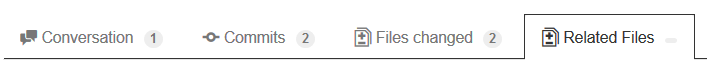
\includegraphics[width=8cm]{NewTabRelatedFiles}
\caption{GitHub pull request page showing the new `Related files' tab}
\label{fig:newTabRelated}
\end{figure}

On opening the tab, a REST~\cite{rest} POST~\cite{post_http} request is sent with the all of the file names from the pull request in its HTTP message body. The REST service, which is deployed on a local instance of a Glassfish server~\cite{glassfish}, receives the file names sent from the GitHub page. The REST service then makes use of the Top-K association rule mining algorithm~\cite{fournier2012mining} to come up with a list of related file names and sends them back to the GitHub page where the request was initiated. The GitHub page will display the results in the 'Related Files' tab as shown in Figure~\ref{fig:relatedFilesContents}. Test files are highlighted in a different color to help developers and reviewers easily distinguish the different types of files. A confidence value is also shown for each file which is obtained from the association rule mining algorithm. Details of the algorithm implementation and the data processing are explained in Section~\ref{sec:dataprocessing}.

\begin{figure}[ht!]
\centering
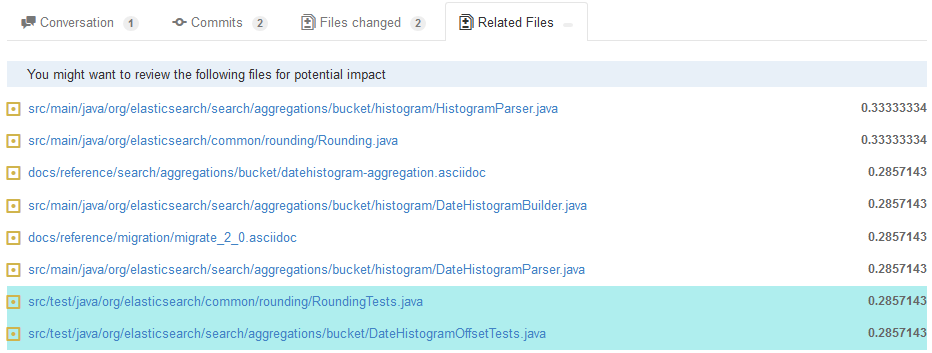
\includegraphics[width=8cm]{RelatedFilesContents}
\caption{`Related files' tab showing files}
\label{fig:relatedFilesContents}
\end{figure}



Figure~\ref{fig:mouseOverOnFile} shows what happens when the mouse is hovered over the hyperlink. It shows the details of the last commit where this file and a changed file in the Pull Request we checked-in together. The same information is shown when the file hyperlink is clicked as well. This helps reviewers to understand why a certain file is there in the list and give them some context on how the file might be impacted.


\begin{figure}[ht!]
\centering
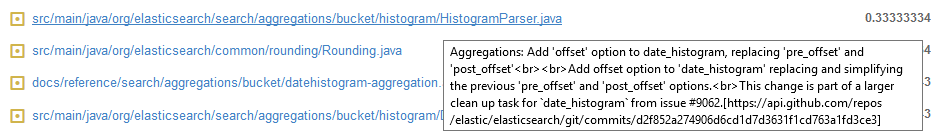
\includegraphics[width=8cm]{MouseOverOfFile}
\caption{Details of the file on performing mouse-over on the hyperlink}
\label{fig:mouseOverOnFile}
\end{figure}

\begin{figure}[ht!]
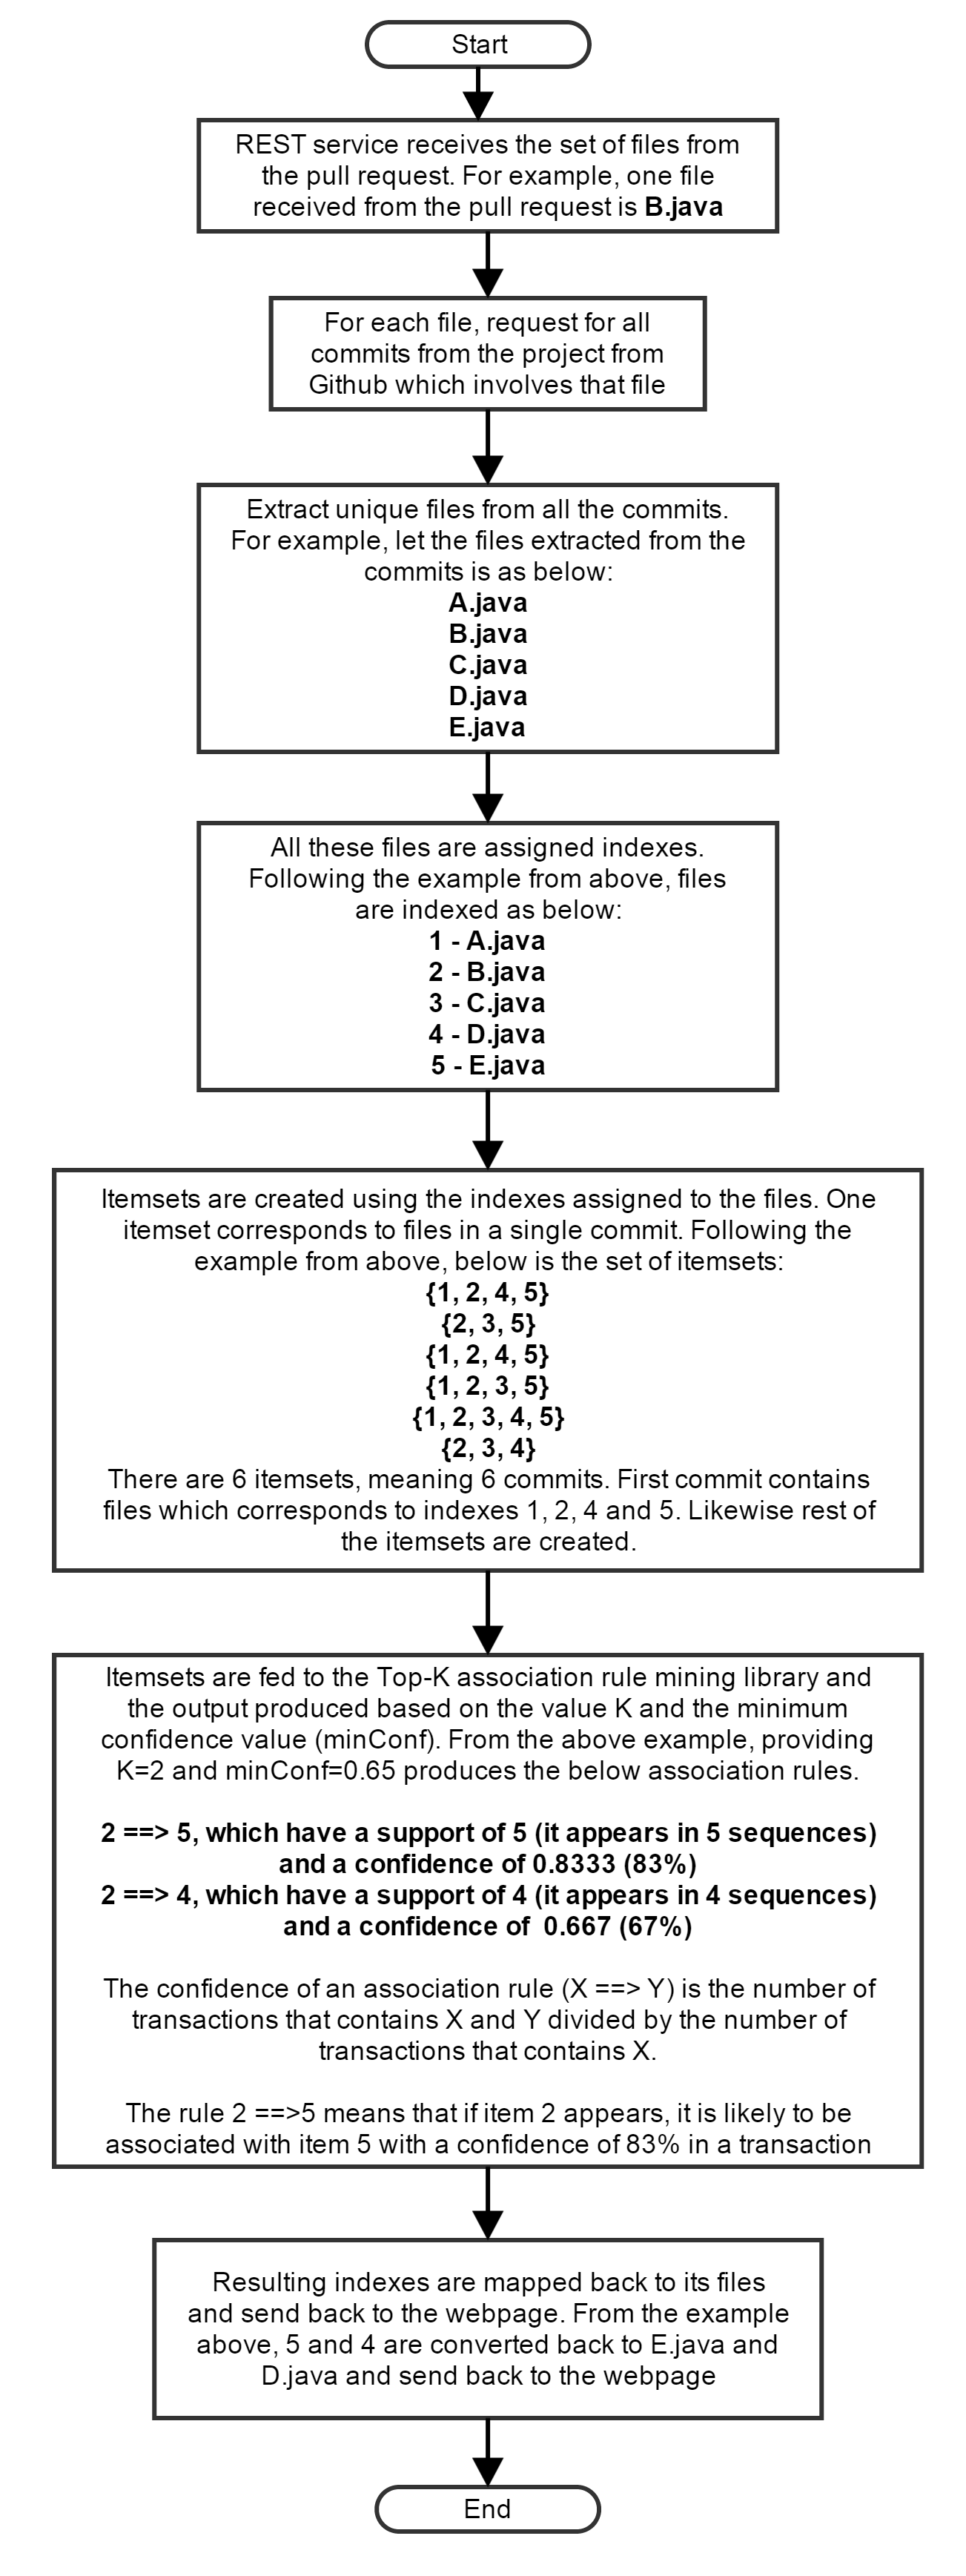
\includegraphics[width=8cm]{data_processing_spmf}
\caption{Data processing process flow with example}
\label{fig:data_processing_spmf}
\end{figure}

\subsection{Data processing}
\label{sec:dataprocessing}

We used the Sequential Pattern Mining Framework (SPMF), an open-source data mining library written in Java~\cite{algo_impl}, which consists of an implementation of the Top-K association rule mining algorithm. We used 10 as the value of K, meaning the library will retrieve at most 10 association rules to be discovered. Another input parameter required by the library is the minimum confidence value. In our case, we provided 0.1 as the minimum confidence value. In order to fit the required format of the data mining library, we needed to perform some data processing to convert the data into the required state.. First, the list of files is received as input to the REST service. Second, using the GitHub API, all of the commits containing these files are retrieved from the particular GitHub project. Third, these initial set of files and the files contained in the commits are assigned indexes, so that each file can be addressed with a number. For example, suppose  we have files named A.java, B.java and C.properties and they are indexed 1, 2 and 3, respectively. This will form a  group of itemsets. Each itemset is a series of distinct numbers which corresponds to the files contained in a particular commit. This group of itemsets are fed into the mining library, which provides the association rules as output. This flow is further explained with an example in Figure~\ref{fig:data_processing_spmf}.
